\section{Multivariate responses}\label{sec:loglin-multiv}

In many studies, there may be \emph{several} categorical responses observed
along with one or more explanatory variables.
In a clinical trial, for example, the efficacy of a drug might be the
primary response, but the occurrence of side-effects might give rise to
additional response variables of substantive interest.
Or, in a study of occupational health, the occurrence of two or more
distinct symptoms might be treated as response variables.

If there are no explanatory variables, then the problem is simply to
understand the joint distribution of the response categories,
and the \loglin\ models and graphical displays described earlier
are sufficient.
Otherwise,
in these cases we usually wish to understand how the various responses
are affected by the explanatory variables.
Moreover, it may also be important to understand how the association
between the categorical responses depends on the explanatory variables.
That is, we would like to study how \emph{both} the marginal distributions
of the responses, and their joint distribution depends on the
predictors.

Although the general \loglin\ model is often used in these situations,
there are special reparameterizations that
may be used to separate the marginal dependence of each response
on the explanatory variables from the interdependence among the responses.


Let us say that categorical responses, $R_1$, $R_2, \dots$ have been
observed, together with possible explanatory variables,
$E_1$, $E_2, \dots$,
and let $\pi_{ij\cdots}$ be the joint probability of all the responses
and explanatory variables;
we also use
$\vec{x}$ to refer to the values of $E_1$, $E_2, \dots$.

Note that the minimal model of independence of all responses from each other
and from the explanatory variables is the \loglin\ model
$[R_1] [R_2] \cdots [E_1 E_2 \cdots]$
(i.e., all associations among the $E_i$ must be included).
A no-effect model, in which the responses do not depend on the
explanatory variables, but may be associated among themselves is
$[R_1 R_2 \cdots] [E_1 E_2 \cdots]$.  However,  these models do not separate
the individual
(marginal) effects of $E_1, E_2 \dots$ on each $R_i$ from their associative effects.

There are three useful general approaches which \emph{do} separate these effects:
\begin{itemize}
\item Model the marginal dependence of each response, $R_i$ separately on $E_1$, $E_2, \dots$,
and, in addition, model the interdependence among the responses.
\item Model the joint dependence of all responses on $E_1$, $E_2, \dots$,
parameterized so that marginal and associative effects are delineated.
\item Construct simultaneous models, estimated together, for the
marginal and joint dependence of the responses on the explanatory variables.
\end{itemize}

The first approach is the simplest, an informative starting place,
and is satisfactory in (the unlikely) case that the responses
are not associated, or if the associations among responses do not vary much
over the explanatory variables (i.e., no terms like $[R_1 R_2 E_j]$ are
required).  In the clinical trial example, we would construct separate
\loglin\ or logit models for efficacy of the drug, and for occurrence
of side-effects, and supplement these analyses with mosaic or other
displays showing the relations between efficacy and side-effects.
This approach is carried out with \PROC{CATMOD} by
using the \pname{RESPONSE LOGITS} statement.

In the second approach, the joint probabilities,  $\pi_{ij\cdots}$,
are recast to give separate information regarding the
dependence of the univariate marginal probabilities
$\pi_{i\bullet}, \pi_{\bullet j}, \dots$,
on the explanatory variables
and the dependence of the intra-response associations on
the explanatory variables.
This approach is carried out by specifying a transformation
of the joint probabilities on the \stmt{RESPONSE}{CATMOD}.

The third approach, exemplified by \citet{LangAgresti:94}
is the most general, but requires specialized software
for model fitting.

Two related models are discussed by \citet[Section 6.5]{McCullaghNelder:89}.
We consider here only the case of two binary responses. Let $\vec{x}$
refer to the values of the explanatory variables and let $\pi _{ij}\left(
\vec{x}\right) $ be the joint probabilities in cell $R_1=i,\,R_2=j$. The
\glossterm{bivariate logistic model} arises from a linear transformation of the
cell probabilities to probabilities $\vec{\gamma }$ which include the
univariate margins, given by
\begin{equation}\label{eq:gamma1}
\vec{\gamma =L\pi }
\end{equation}
where $\mat{L}$ is a matrix of 0s and 1s of the form of a factorial
design matrix transposed. In the $2\times 2$ case,
\begin{equation}\label{eq:gamma2}
\vec{\gamma =}\left(
\begin{array}{c}
\pi _{1\bullet } \\
\pi _{2\bullet } \\
\pi _{\bullet 1} \\
\pi _{\bullet 2} \\
\pi _{11} \\
\pi _{12} \\
\pi _{21} \\
\pi _{22}
\end{array}
\right) =\left[
\begin{array}{cccc}
1 & 1 & 0 & 0 \\
0 & 0 & 1 & 1 \\
1 & 0 & 1 & 0 \\
0 & 1 & 0 & 1 \\
1 & 0 & 0 & 0 \\
0 & 1 & 0 & 0 \\
0 & 0 & 1 & 0 \\
0 & 0 & 0 & 1
\end{array}
\right] \left(
\begin{array}{c}
\pi _{11} \\
\pi _{12} \\
\pi _{21} \\
\pi _{22}
\end{array}
\right)
\end{equation}

There are of course only three linearly independent probabilities, because $%
\sum \sum \pi _{ij}=1$. The bivariate logistic model is formulated in terms
of factorial contrasts on the elements of $\vec{\gamma }$ which express
separate models for the two logits and the log odds. The model is expressed
as
\begin{equation*}%\label{eq:eta1}
 \vec{\eta }=\mat{C}\log \vec{\gamma =\mat{C}}\log \mat{L \pi}
 \comma
\end{equation*}
where $\mat{C}$ is a matrix of contrasts. In the $2\times 2$ case, the
usual contrasts may be defined by
\begin{equation}\label{eq:eta2}
\vec{\eta }=\left(
\begin{array}{c}
\eta _1 \\
\eta _2 \\
\eta _{12}
\end{array}
\right) =\left(
\begin{array}{c}
\mathrm{logit}\;\pi _{1\bullet } \\
\mathrm{logit}\;\pi _{\bullet 1} \\
\mathrm{\theta}
\end{array}
\right) =\left[
\begin{array}{rrrrrrrr}
1 & -1 & 0 & 0 & 0 & 0 & 0 & 0 \\
0 &  0 & 1 & -1 & 0 & 0 & 0 & 0 \\
0 &  0 & 0 & 0 & 1 & -1 & -1 & 1
\end{array}
\right] \left(
\begin{array}{c}
\pi _{1\bullet } \\
\pi _{2\bullet } \\
\pi _{\bullet 1} \\
\pi _{\bullet 2} \\
\pi _{11} \\
\pi _{12} \\
\pi _{21} \\
\pi _{22}
\end{array}
\right)
\end{equation}
Thus, we are modeling the marginal odds of each response, together
with the log odds ratio $theta$ simultaneously.

Specific models are then formulated for the dependence of $\eta _1\left( \vec{x}%
\right) ,\eta _2\left( \vec{x}\right) $ and $\eta _{12}\left( \vec{x}%
\right) $ on the explanatory variables. For example, with one quantitative
explanatory variable, $x$, the model
\begin{equation}\label{eq:bilogit1}
\left(
\begin{array}{c}
\eta _1 \\
\eta _2 \\
\eta _{12}
\end{array}
\right) =\left(
\begin{array}{c}
\alpha _1+\beta _1 x \\
\alpha _2+\beta _2 x \\
\theta
\end{array}
\right)
\end{equation}
asserts that the log odds of each response changes linearly with $x$, while
the odds ratio between the responses remains constant. In the general form
given by \cite{McCullaghNelder:89} the submodels in \eqref{eq:bilogit1} may
each depend on the explanatory variables in different ways.
For example, the logits could both depend quadratically on $x$,
while an intercept-only model could be posited for the log odds ratio.

In \PROC{CATMOD} such general models can only be tested by specifying the
design matrix directly in the \stmt{MODEL}{CATMOD}.  The matrices $\mat{L}$ and $\mat{C}$ in
\eqref{eq:gamma2} and \eqref{eq:eta2} are specified on the \stmt{RESPONSE}{CATMOD}.

The second model is a \glossterm{bivariate loglinear model}, obtained by taking
$\mat{L}=\mat{I}$ in \eqref{eq:gamma1}, so that $\vec{\gamma} = \vec{\pi}$.
Then a \loglin\ model of the form
\begin{equation*}
\vec{\eta } ( \vec{x} ) = \mat{C} \log \vec{\pi}
\end{equation*}
expresses contrasts among log probabilities as linear functions of
the explanatory variables.  For the $2 \times 2$ case, we take the
contrasts as
\begin{equation}\label{eq:eta3}
 \vec{\eta }=\left(
 \begin{array}{c}
  l_1 \\
  l_2 \\
  \eta _{12}
 \end{array}
 \right) =\left[
 \begin{array}{rrrr}
  1 & 1 & -1 & -1 \\
  1 & -1 & 1 & -1 \\
  1 & -1 & 1 & -1
 \end{array}
\right] \left(
 \begin{array}{c}
  \log \,\pi _{11} \\
  \log \,\pi _{12} \\
  \log \,\pi _{21} \\
  \log \,\pi _{22}
 \end{array}
\right)
\end{equation}
and models for the dependence of $l _1\left( \vec{x}%
\right) , l _2\left( \vec{x}\right) $ and $\eta _{12}\left( \vec{x}%
\right) $ are expressed in the same way as \eqref{eq:bilogit1}.
The estimates of the odds ratio, $\eta _{12}$ are the same under both
models.  The marginal functions are parameterized differently, however,
but lead to similar predicted probabilities.
The fitting and graphing of these models is illustrated in the
next example.

\begin{Example}[ashford]{Breathlessness and wheeze in coal miners}
In \exref{ex:wheeze1} we examined the association between the occurrence
of two pulmonary conditions, breathlessness and wheeze,
among coal miners, classified by age \citep{AshfordSnowden:70}.
\figref{fig:pie2x2wh1} showed fourfold displays focused on the odds ratio
for the co-occurrence of these symptoms,
and \figref{fig:pie2x2wh2} plotted these odds ratios against age directly.
Here, we consider models which examine the changes in prevalence of
the two symptoms over age, together with the changes in their association.

As a first step, we calculate the log odds for breathlessness and for
wheeze, and the log odds ratio for their association
in each $2 \times 2$ table. These values are shown in \outref{out:ashford.1}.
The log odds ratios are the same values plotted in \figref{fig:pie2x2wh2}
(but the youngest age group was not included in the earlier analysis).
\begin{listing}
data ashford;
   input age @;
   age2 = age**2;
   do breath = 1, 0;
      do wheeze = 1, 0;
         input count @;
         output;
         end;
      end;
   label breath='Breathlessness'
      wheeze='Wheeze'
      age='Age Group';
datalines;
20     9    7      95 1841
25    23    9     105 1654
30    54   19     177 1863
35   121   48     257 2357
40   169   54     273 1778
45   269   88     324 1712
50   404  117     245 1324
55   406  152     225  967
60   372  106     132  526
;
proc transpose out=ashford1 prefix=r;
   var count;
   by age;

data ashford1;
   set ashford1;
   drop _name_;
   logit1 = log( (r1 + r2 + .5) / (r3 + r4 + .5) );
   logit2 = log( (r1 + r3 + .5) / (r2 + r4 + .5) );
   logodds= log( ((r1+.5)*(r4+.5))/((r2+.5)*(r3+.5)) );
   label logit1='Logit(Breathlessness)'
      logit2='Logit(Wheeze)';
proc print;  id age;
\end{listing}

\begin{Output}[htb]
\caption{Empirical logits and log odds ratios for breathlessness and wheeze}\label{out:ashford.1}
\small
\verbatiminput{ch7/out/ashford.1}
\end{Output}

Plotting both logits and the log odds against age gives the graph shown
in \figref{fig:ashford1}.
The plotting step is straight-forward and is not shown.
We see that both symptoms, while quite rare among young miners, increase
steadily with age (or years working in the mine).
There is a hint of curvilinearity, particularly in the logit for
breathlessness.
The decline in the odds ratio with age reflects selection, as miners
who had retired for health or other reasons were excluded from the
study.
%% one figure
\begin{figure}[htb]
  \centering
  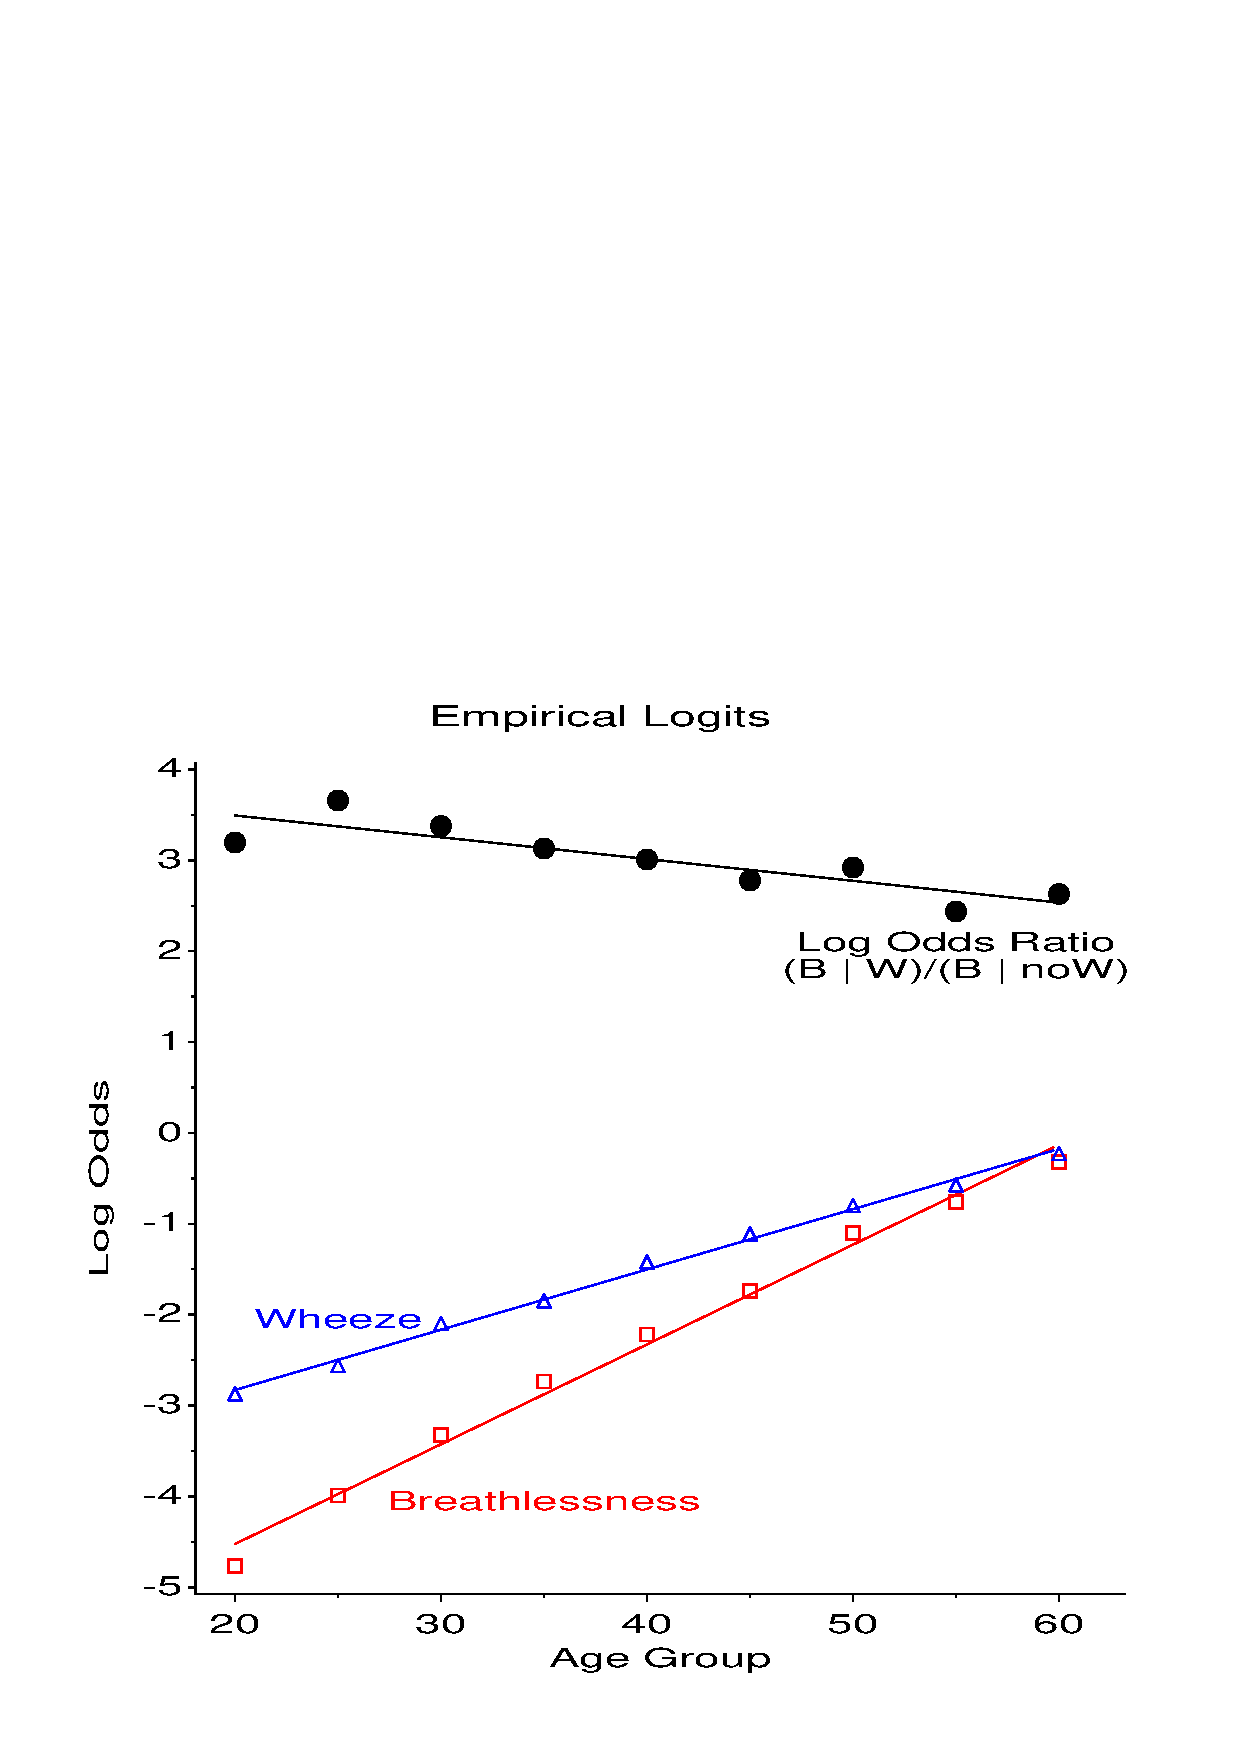
\includegraphics[scale=.6]{ashford1}
  \caption[Empirical logits and log odds ratios for breathlessness and wheeze]{Empirical logits and log odds ratios for breathlessness and wheeze.
  The lines show separate linear regressions for each function.}%
  \label{fig:ashford1}
\end{figure}

We can fit ordinary \loglin\ models to these data as shown below,
giving \LR\ goodness-of-fit \GSQ\ values shown in \tabref{tab:ashmod}.
Note that in Models 0--2, age is treated as a 9-level factor.
In Models 3--4, age is treated as a quantitative variable
(symbolized as $x$ in the model terms), by declaring
\pname{age} and \pname{age2} ($x^2$) in a \stmt{DIRECT}{CATMOD}.%
\footnote{In these model formulae, a term like $[Bx^2]$
refers to a quadratic model, $\eta_1 = \alpha_1 + \beta_{11} x + \beta_{11} x^2$ in \eqref{eq:bilogit1}}
\PROC{CATMOD} does not allow quantitative variables to appear
on the left-hand side in a \stmt{MODEL}{CATMOD}.
Consequently, these models are fit in a separate \PROC{CATMOD}
step, where they are expressed as \verb|_RESPONSE_*AGE| and
\verb|_RESPONSE_*AGE2| on the right-hand side.
%% input: /users/faculty/friendly/sasuser/catdata/ash1.sas
%% last modified: 16-Nov-98 13:44
\begin{listing}
title 'Loglinear models for B and W';   
proc catmod order=data data=ashford;
   weight count;
   model breath*wheeze*age = _response_ / 
      ml noiter noresponse noprofile nodesign nogls;
   loglin breath wheeze age / title='0: Minimal model: [B] [W] [A]';
run;
   loglin breath|wheeze age / title='1: Null age: [BW] [A]';
run;
   loglin breath|wheeze breath|age wheeze|age/ title='2: [BW] [BA] [WA]';

proc catmod order=data data=ashford;
   weight count;
   direct age age2;
   model breath*wheeze = _response_ _response_*age/ 
      ml noiter noresponse noprofile nodesign nogls;
   loglin breath|wheeze / title='3: [BW] [Bx] [Wx]';
run;
   model breath*wheeze = _response_ _response_*age _response_*age2/ 
      ml noiter noresponse noprofile nodesign nogls;
   loglin breath|wheeze / title='4: [BW] [Bx^2] [Wx^2]';
run;

\end{listing}

%\begin{table}[htb]
% \caption{Loglinear models fit to Ashford \& Snowden data}\label{tab:ashmod}
% \begin{center}
% \begin{tabular}{cl rrrr}
%  \hline
%  Model & Terms            & df & \GSQ & $p$-value & \GSQ /df \\ 
%  \hline
%  0 & $[B]  [W]  [A]$      & 25 & 6939.07 & 0.0000 & 277.56 \\ 
%  1 & $[BW] [A]$           & 24 & 2701.94 & 0.0000 & 112.58 \\ 
%  2 & $[BW] [BA] [WA]$     &  8 & 26.69   & 0.0008 & 3.34 \\ 
%  3 & $[BW] [Bx] [Wx]$     & 21 & 41.46   & 0.0049 & 1.97 \\ 
%  4 & $[BW] [Bx^2] [Wx^2]$ & 18 & 17.60   & 0.4825 & 0.97 \\ 
%  \hline
% \end{tabular}
% \end{center}
%\end{table}
%

% latex table generated in R 3.0.1 by xtable 1.7-3 package
% Thu May 08 11:49:32 2014
\begin{table}[htb]
 \caption{Loglinear models \func{glm} fit to Ashford \& Sowden data}\label{tab:ashmod}
\centering
\begin{tabular}{rlrrrrr}
  \hline
  Model   & Terms & LR Chisq & \GSQ & Pr($>$Chisq) & AIC & BIC \\ 
  \hline
  cm.glm0 & $\LLM{B, W, A}$ & 6939.07 & 25 & 0.0000 & 6889.07 & 6693.73 \\ 
  cm.glm1 & $\LLM{BW, A}$ & 2701.94 & 24 & 0.0000 & 2653.94 & 2466.42 \\ 
  cm.glm2 & $\LLM{BW,BA,WA}$ & 26.69 & 8 & 0.0008 & 10.69 & -51.82 \\ 
  cm.glm3 & $\LLM{BWx,BA,WA}$ & 6.80 & 7 & 0.4498 & -7.20 & -61.89 \\ 
   \hline
\end{tabular}
\end{table}



Model 0 is the minimal model of mutual independence; Model 1 allows
association of breathlessness and wheeze, but independent of age.
Neither of these makes any sense, given what we have seen graphically.
Model 2 allows both breathlessness and wheeze to depend on age as a factor.
The quantitative models for age, Models 3 and 4
correspond to what is apparent in \figref{fig:ashford1}.
Model 3 is equivalent in goodness-of-fit
to the bivariate \loglin\ model \eqref{eq:eta3},
but is parameterized in terms of generalized logits
\begin{equation*}
\left(
\begin{array}{c}
l _{11,22} \\
l _{12,22} \\
l _{21,22}
\end{array}
\right) =
\left(
\begin{array}{c}
\log \pi_{11} / \pi_{22} \\
\log \pi_{12} / \pi_{22} \\
\log \pi_{21} / \pi_{22}
\end{array}
\right) =
\left(
\begin{array}{c}
\alpha _1+\beta _1 x \\
\alpha _2+\beta _2 x \\
\alpha _{12}+\beta _{12} x \\
\end{array}
\right)   %\label{eq:biloglin}
\period
\end{equation*}
Model 4 adds terms in $x^2$ to each of these equations.
From the \GSQ\  and \GSQ/df values in \tabref{tab:ashmod} it appears that
only Model 4 is acceptable.

Loglinear models parameterized as in \eqref{eq:eta3} may be fit by
specifying the logit contrasts shown there
in the \stmt{RESPONSE}{CATMOD}.
For instance, the following model has the same \GSQ\ as
Model 3, but the fitted function values are those of $\hat{l}_1$,
$\hat{l}_2$ and the odds ratio
$\hat{\eta}_{12}$.
\begin{listing}
proc catmod order=data data=ashford;
   direct age ;
   weight count;
   response  1  1 -1 -1,
             1 -1  1 -1,
             1 -1 -1  1  log / out=predict;
   model breath*wheeze = age  /  noiter nogls prob noprofile;
   title '[BW] [Bx] [Wx], Loglinear, logit contrasts';
\end{listing}

The bivariate logit model is more complex because the \stmt{RESPONSE}{CATMOD}
must include both the $\mat{L}$ matrix from \eqref{eq:gamma2} and the $\mat{C}$ matrix from \eqref{eq:gamma2}.
Nevertheless, the fitted functions correspond exactly to
what is plotted in \figref{fig:ashford1}.
Model fit statistics and the parameter estimates for the linear model
are shown in \outref{out:ashford.2}.
%% input: /users/faculty/friendly/sasuser/catdata/ash2.sas
%% last modified: 16-Nov-98 16:04
\begin{listing}
proc catmod order=data data=ashford;
   direct age ;
   weight count;
   response                      /* C matrix */
     1 -1  0  0  0  0  0  0,     /* logit1 */
     0  0  1 -1  0  0  0  0,     /* logit2 */
     0  0  0  0  1 -1 -1  1      /* logodds */
      log
        1  1  0  0,              /* L matrix */
        0  0  1  1,
        1  0  1  0,
        0  1  0  1,
        1  0  0  0,
        0  1  0  0,
        0  0  1  0,
        0  0  0  1 / out=predict;                       
   model breath*wheeze = age  /  noiter nogls;
   title '[BW] [Bx] [Wx], Bivariate logit model';

\end{listing}

%% one figure
\begin{figure}[htb]
  \centering
  \includegraphics[scale=.6]{ash21}
  \caption[Observed and fitted logits and log odds ratios, linear bivariate model]{Observed (points) and fitted (lines) logits and log odds ratios for  the linear bivariate logit model}%
  \label{fig:ash21}
\end{figure}

The observed and fitted function values (the logits and odds ratio)
are plotted as shown below, giving the graph in \figref{fig:ash21}.
The fitted relations are very similar to those shown in \figref{fig:ashford1},
although the models for the marginal functions are
parameterized quite differently.

%% input: /users/faculty/friendly/sasuser/catdata/ash2.sas
%% last modified: 17-Nov-98 10:55
\begin{listing}
proc sort data=predict;
   where (_type_='FUNCTION');
   by _number_;
%label(data=predict, x=age, y=_pred_, 
   color=scan('red blue black', _number_),
   text=scan('Breathlessness Wheeze Odds_Ratio', _number_),
   pos=scan('9 1 3', _number_), subset=(age=35), out=_lab_);
%points(data=predict, x=age, y=_obs_,
   color=scan('red blue black', _number_),
   symbol=scan('square triangle dot', _number_), size=2, out=_pts_);
data _anno_;
   set _lab_ _pts_;

proc gplot data=predict;
   plot  _pred_ * age = _number_ /
        vaxis=axis1 vm=1 hm=1 haxis=axis2 anno=_anno_ nolegend;
   symbol1 v=none i=join c=red;
   symbol2 v=none i=join c=blue;
   symbol3 v=none i=join c=black;
   axis1 label=(a=90) order=(-5 to 4) offset=(4);
   axis2 offset=(3,5);
   label _pred_ = 'Log Odds';
\end{listing}

The quadratic model, corresponding to Model 4 may be fit and plotted
exactly in the same way, changing the \stmt{MODEL}{CATMOD} in the lines above to
\begin{listing}
   model breath*wheeze = age age2;
\end{listing}
where \pname{age2} has also been declared in the \stmt{DIRECT}{CATMOD}.
The quadratic model is graphed in \figref{fig:ash22}.
The model fit statistics for these bivariate logit models
(\tabref{tab:ashmod2}) indicate that both models fit better than their
\loglin\ counterparts.  The table also shows an intermediate model,
Model 4m, which was fit by specifying the design matrix numerically
in the \stmt{MODEL}{CATMOD}.  In this model, the log odds ratio has
only a linear term in age, while breathlessness and wheeze vary
quadratically.

\begin{table}[htb]
 \caption{Bivariate logit models fit to Ashford \& Snowden data}\label{tab:ashmod2}
 \begin{center}
 \begin{tabular}{cl rrrr}
  \hline
  Model & Terms            & df & \chisq & $p$-value & \chisq/df \\ 
  \hline
  3 & $ [BWx] [Bx] [Wx]$      & 21 & 30.15  & 0.0890 & 1.44 \\ 
  4m & $[BWx] [Bx^2] [Wx^2]$  & 19 & 17.07  & 0.5853 & 0.94 \\
  4 & $[BWx^2] [Bx^2] [Wx^2]$ & 18 & 16.94  &  0.5270 & 0.94 \\ 
  \hline
 \end{tabular}
 \end{center}
\end{table}


%% one figure
\begin{figure}[htb]
  \centering
  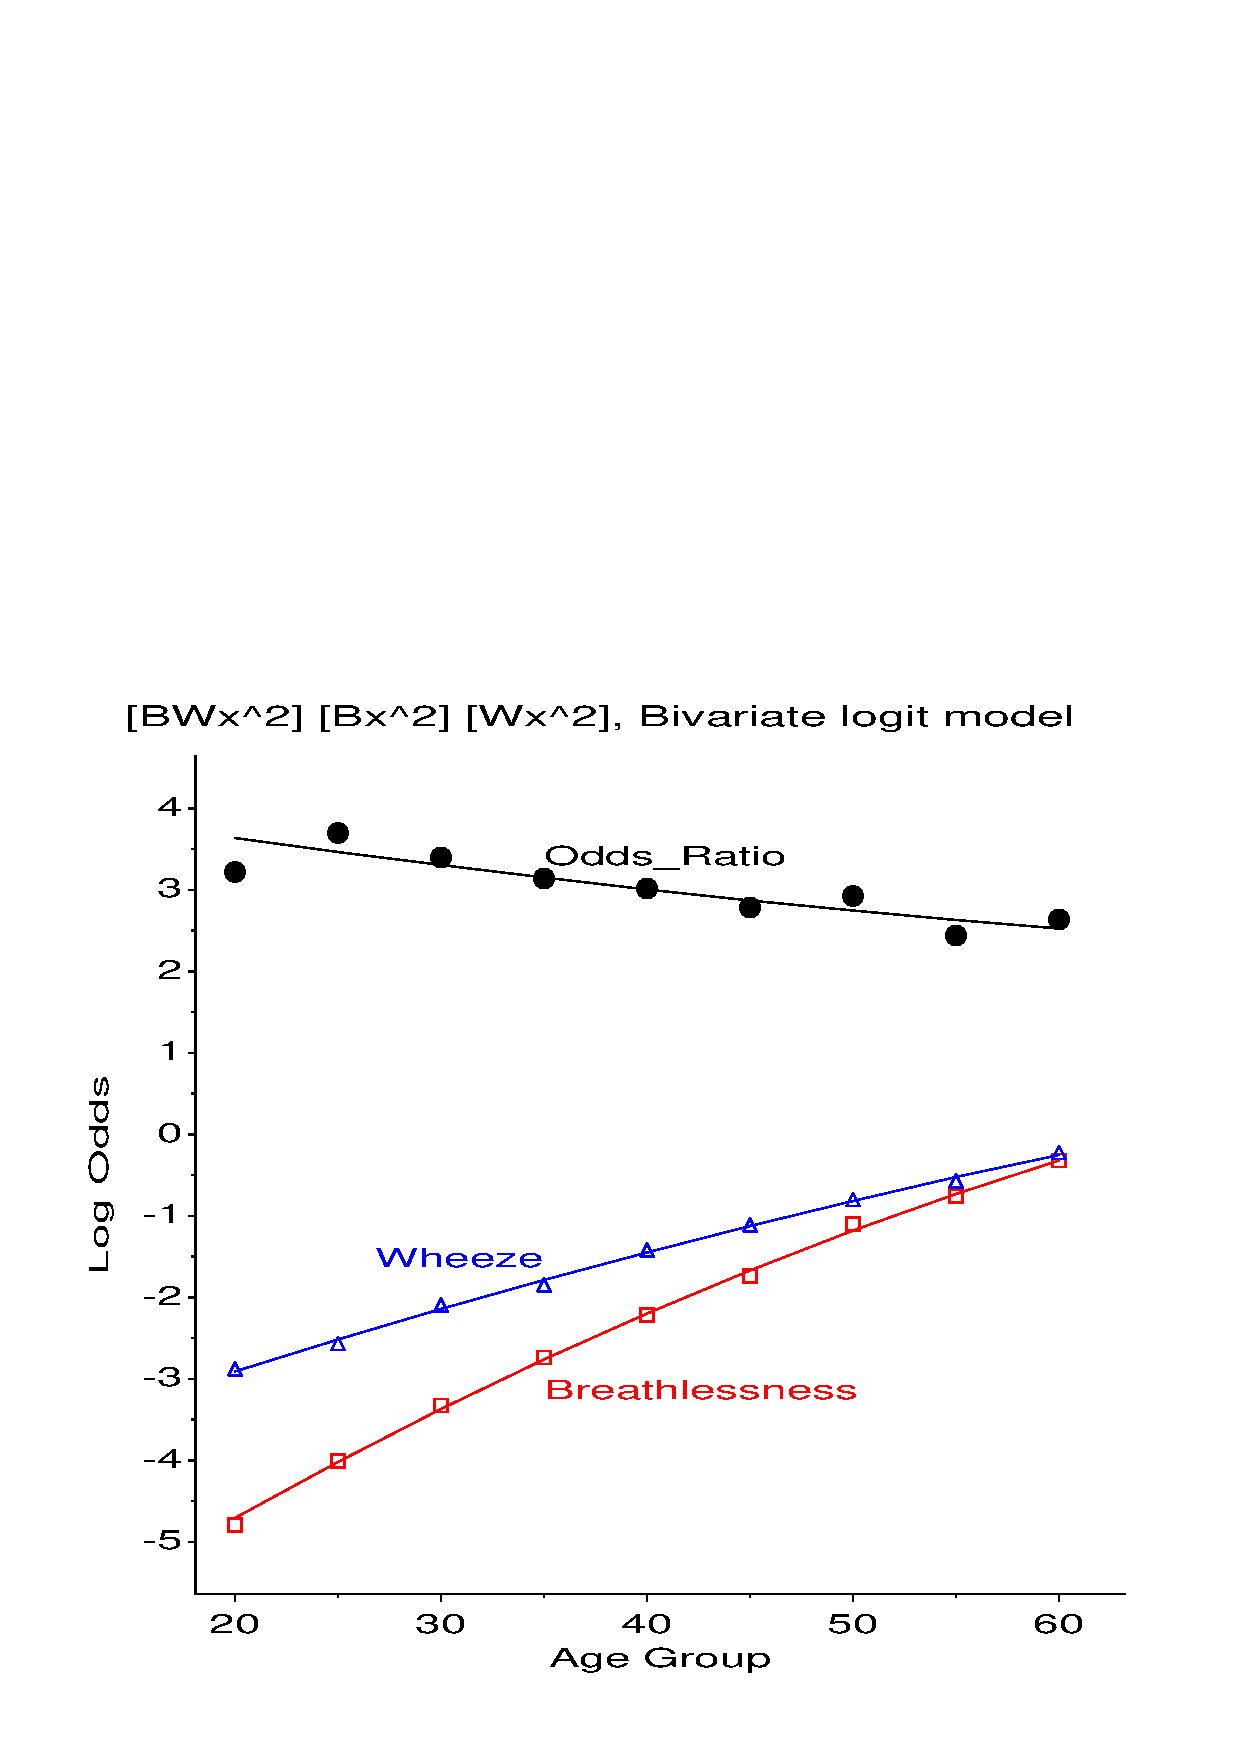
\includegraphics[scale=.6]{ash22}
  \caption[Observed and fitted logits and log odds ratios, quadratic model]{Observed (points) and fitted (curves) logits and log odds ratios for quadratic bivariate logit model}%
  \label{fig:ash22}
\end{figure}

\begin{Output}[htb]
\caption{Model fit and parameter estimates for the linear bivariate logit model }\label{out:ashford.2}
\small
\verbatiminput{ch7/out/ashford.2}
\end{Output}
On statistical grounds, we might be led to choose the quadratic model
as the best fit, but the graphical evidence suggests that the difference
between them is slight.
\figref{fig:ash21} and \figref{fig:ash22} are also both quite similar to the plot
of the empirical logits in \figref{fig:ashford1}, but the fitted models
give a simplified description.
Thus, Model 3 may be summarized as
\begin{equation*}
\left(
\begin{array}{c}
\eta _B \\
\eta _W \\
\eta _{BW}
\end{array}
\right) =\left(
\begin{array}{r}
-6.354 + 0.102 \mbox{ age} \\
-4.089 + 0.065 \mbox{ age} \\
 4.066 - 0.026 \mbox{ age} \\
\end{array}
\right)
\end{equation*}
For each five years, the odds of a miner showing breathlessness are
multiplied by $\exp (5 \times 0.102) = 1.67$, a 67\% increase;
the odds of wheeze increase by  $\exp (5 \times 0.065) = 1.38$, a 38\%
increase.
\end{Example}


\subsection{Examining relations}
When there is more than one explanatory variable and several responses,
it is useful to begin with a more thorough
visual examination of the relations within and between these sets.
Some useful graphical displays include
\begin{itemize}
\item mosaic displays showing the marginal relations among the response variables
and of the explanatory variables, each collapsed over the other set;
\item partial mosaics or fourfold displays of the associations among
the responses, stratified by one or more of the explanatory variables;
\item plots of empirical logits and log odds ratios, as in \figref{fig:ashford1}.
\end{itemize}
These displays can, and should, inform our search for an adequate
descriptive model.
\begin{Example}[toxaemia]{Toxaemic symptoms in pregnancy}
\citet{Brown-etal:83} gave the data in \tabref{tab:toxtab}
on the occurrence of signs of toxaemia (hypertension and protein urea)
among 13,384 expectant mothers in Bradford, England in their first pregnancy.
The mothers are classified by social class, and by the
number of cigarettes smoked per day.
There are thus two response variables, and two explanatory variables
in this $2 \times 2 \times 5 \times 3$ table.
\begin{table}[htb]
 \caption{Toxaemic symptoms of mothers during pregnancy. From: }\label{tab:toxtab}
 \begin{center}
 \begin{tabular}{c| rrrr| rrrr| rrrr}
  \hline
\multicolumn{1}{r|}{Smoking}
    & \multicolumn{4}{c|}{0} & \multicolumn{4}{c|}{1-19} & \multicolumn{4}{c}{20+} \\

\multicolumn{1}{r|}{Hypertension}
    & \multicolumn{2}{c}{Yes} & \multicolumn{2}{c|}{No} & \multicolumn{2}{c}{Yes} & \multicolumn{2}{c|}{No}  & \multicolumn{2}{c}{Yes} & \multicolumn{2}{c}{No} \\
\multicolumn{1}{r|}{Protein urea}
    & Yes & No & Yes & No & Yes & No & Yes & No & Yes & No & Yes & No \\ 
  \hline
Social Class \\
  \hline
  1 &  28 &   82 &  21 &  286 &   5 &  24 &   5 &   71 &  1 &  3 &  0 & 13 \\ 
  2 &  50 &  266 &  34 &  785 &  13 &  92 &  17 &  284 &  0 & 15 &  3 & 34 \\ 
  3 & 278 & 1101 & 164 & 3160 & 120 & 492 & 142 & 2300 & 16 & 92 & 32 & 383 \\ 
  4 &  63 &  213 &  52 &  656 &  35 & 129 &  46 &  649 &  7 & 40 & 12 & 163 \\ 
  5 &  20 &   78 &  23 &  245 &  22 &  74 &  34 &  321 &  7 & 14 &  4 & 65 \\ 
  \hline
 \end{tabular}
 \end{center}
\end{table}


The questions of main interest are how the occurrence of each symptom
varies with class and smoking, and how the association between them
varies. It is useful, however, to examine first the marginal relationship between
the two responses, and between the two predictors.
These are produced with the \macro{mosaic} as shown below.
The parameter \pname{PLOTS=2} gives a plot of the first two variables,
according to the order in which the data are sorted.
Re-sorting to make \pname{hyper} and \pname{urea} vary most rapidly
gives the second plot.  Both plots are shown in \figref{fig:tox41}.
\begin{listing}
%include catdata(toxaemia);

data toxaemia;
   set toxaemia;
   sm = put(smoke, smoke.);

%mosaic(data=toxaemia, var=Class Sm Hyper Urea, plots=2, htext=2,
   title=%str(Predictors: Class, Smoke));

proc sort data=toxaemia;
   by class sm descending urea descending hyper;
%mosaic(data=toxaemia, var= Hyper Urea Sm Class, plots=2, sort=no, htext=2,
   title=%str(Hypertension and Protein Urea));
\end{listing}

%% one figure
\begin{figure}[htb]
  \centering
  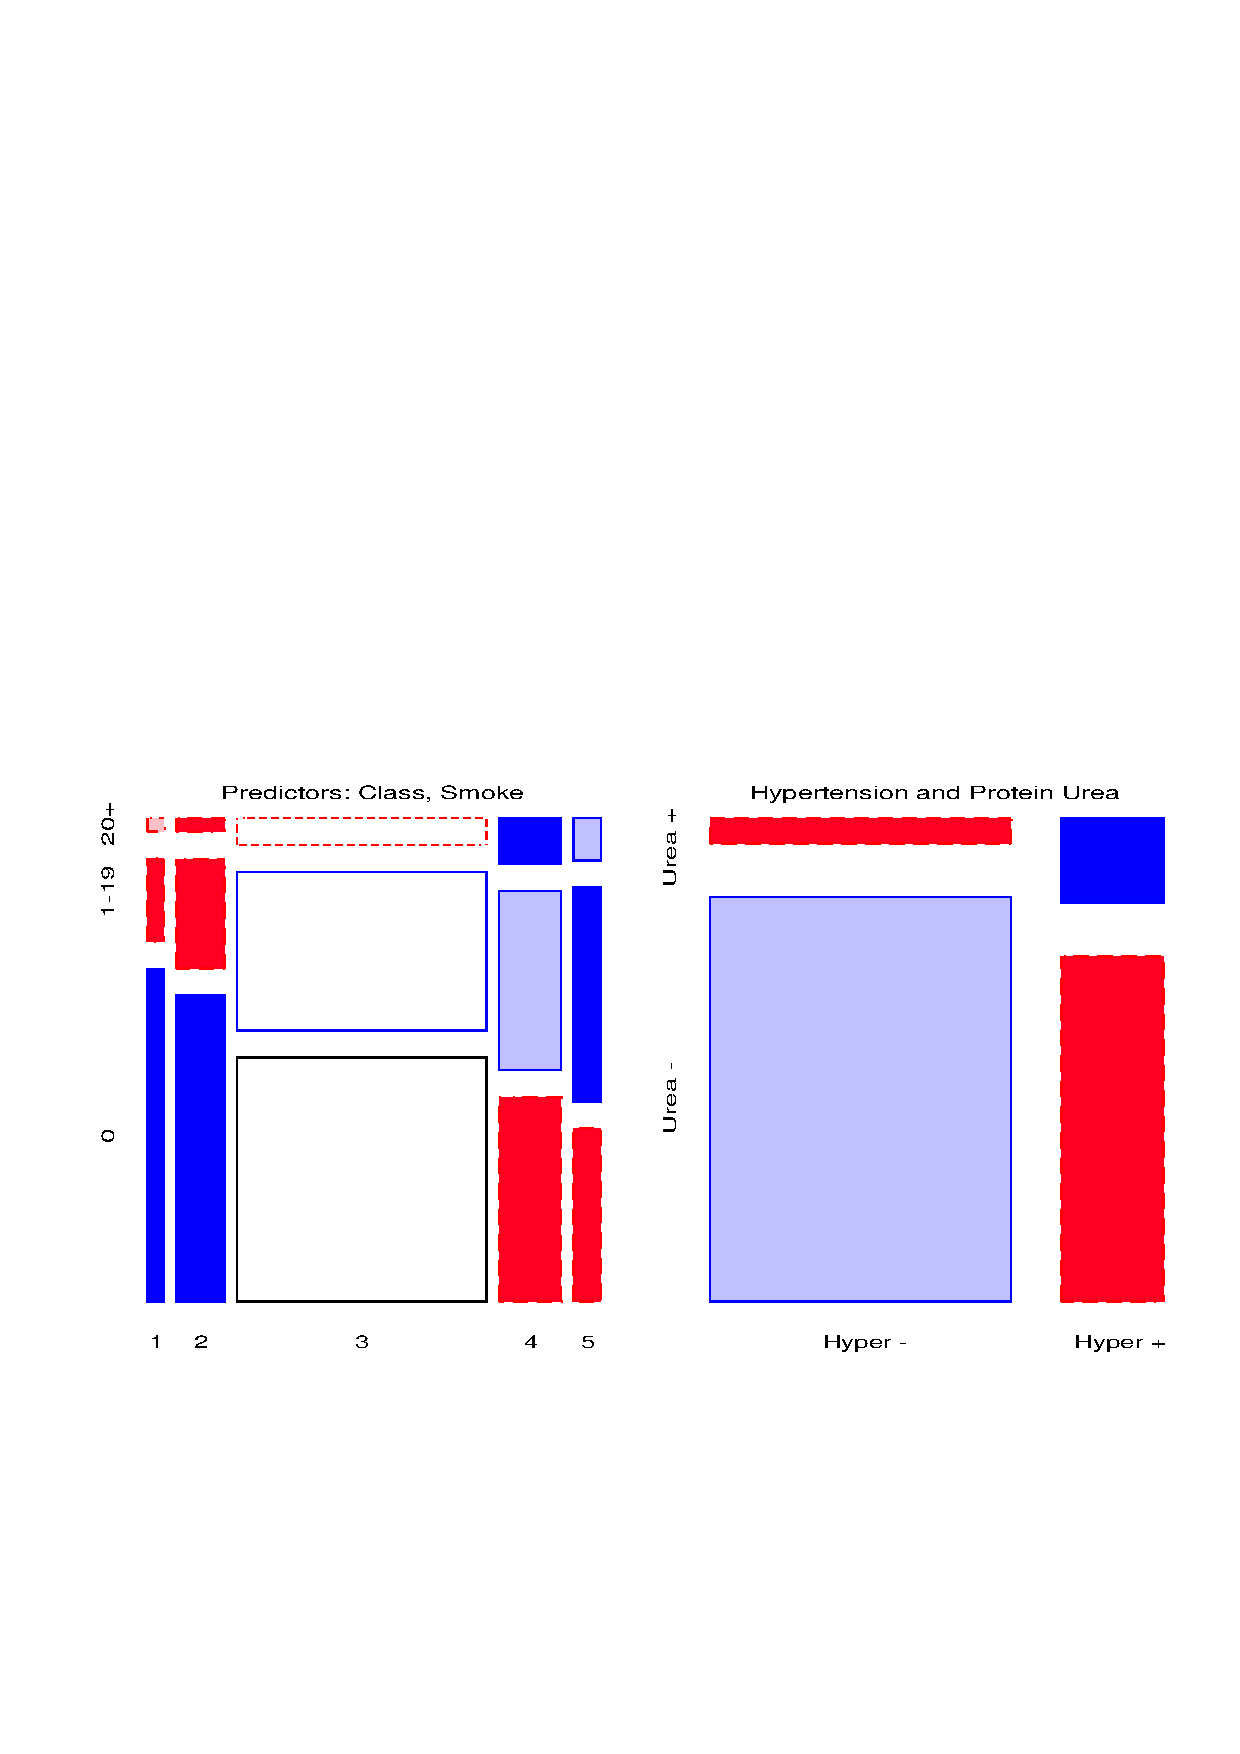
\includegraphics[scale=.6,clip]{tox41}
  \caption{Mosaic displays for toxaemia data: Predictor and Response associations}%
  \label{fig:tox41}
\end{figure}
We see in \figref{fig:tox41} that the majority of the mothers are in the
third social class, and that smoking is negatively related to social
class, with the highest levels of smoking in classes 4 and 5.
Within the responses, the great majority of women exhibit neither symptom,
but showing one symptom makes it more likely to show the other.
Marginally, hypertension is somewhat more prevalent than protein urea.

We next examine how the association between responses varies with
social class and with smoking.
\figref{fig:tox42}  shows a collection of partial
mosaic plots of the association between hypertension and urea,
for each level of smoking, collapsed over social class.
\figref{fig:tox43} is similar, but stratified by social class.
These statements produce \figref{fig:tox42}:
\begin{listing}
proc freq data=toxaemia order=data;
   tables hyper * urea * smoke / out=sum1;
   weight count;
%mosaic(data=sum1,  var= Hyper Urea Smoke, sort=no, by=Smoke, htext=3);
\end{listing}

Ignoring social class, the association between hypertension and protein urea
decreases with smoking.
Ignoring smoking, the association is greatest in social class 3.
However, these two symptoms are positively associated in all cases.

%% one figure
\begin{figure}[htb]
  \centering
  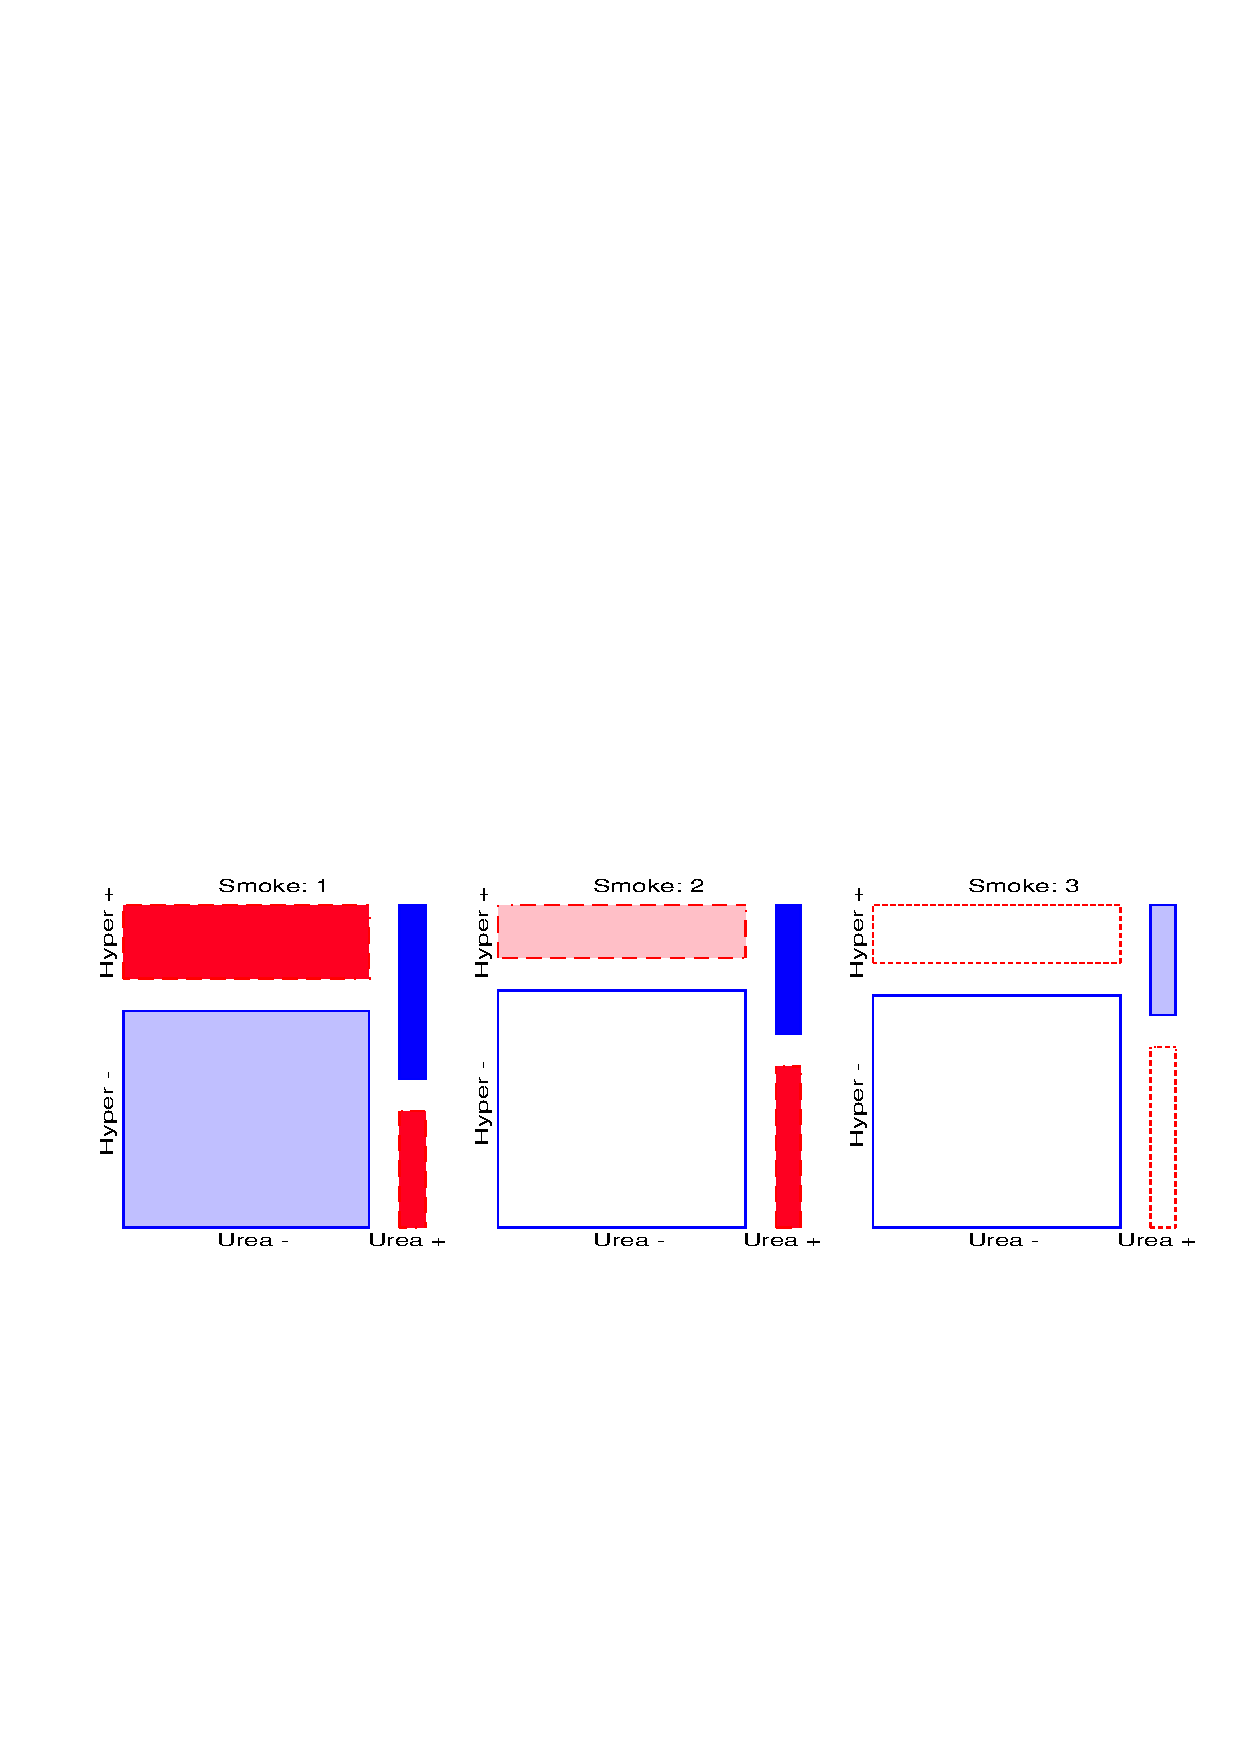
\includegraphics[scale=.75,clip]{tox42}
  \caption{Toxaemia data: Response associations by Smoking}%
  \label{fig:tox42}
\end{figure}
%% one figure
\begin{figure}[htb]
  \centering
  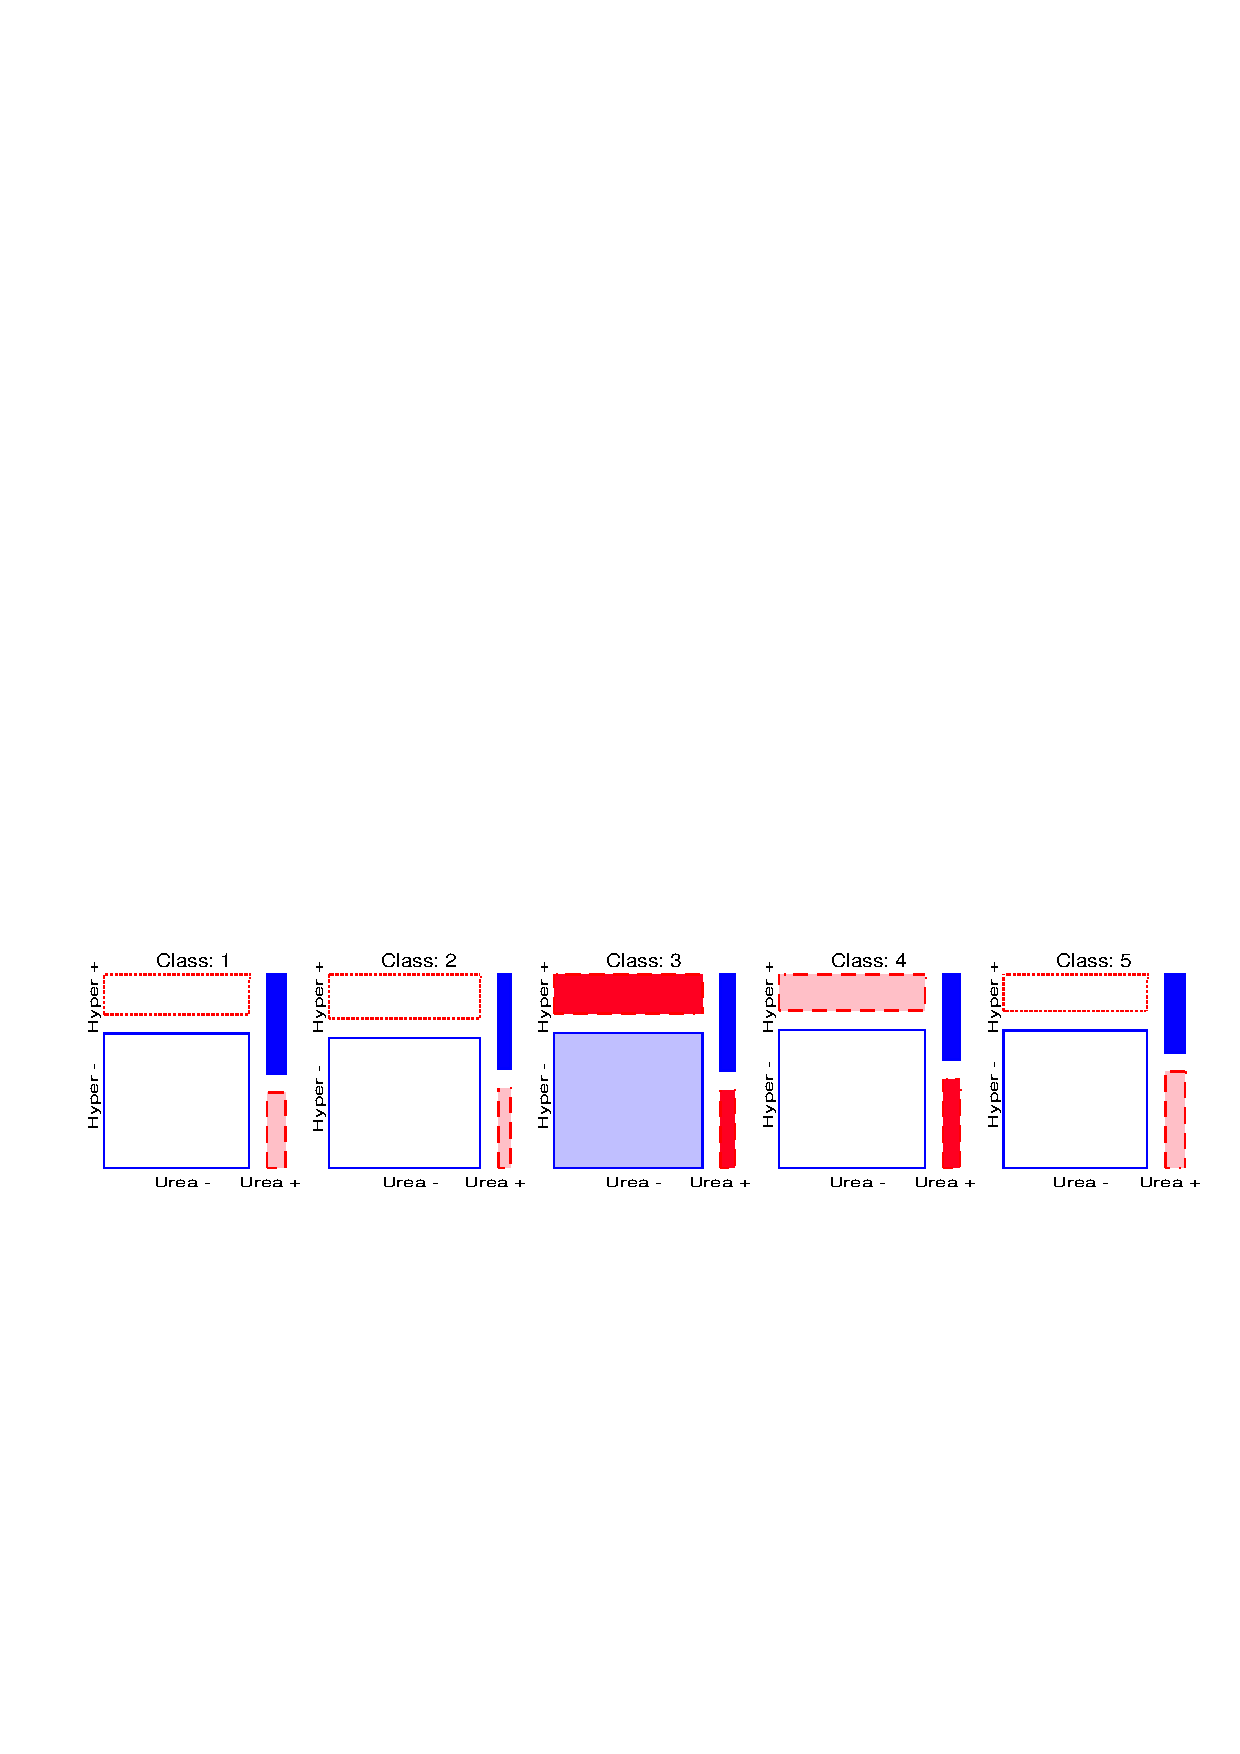
\includegraphics[scale=.75,clip]{tox43}
  \caption{Toxaemia data: Response associations by Social Class}%
  \label{fig:tox43}
\end{figure}

Our initial overview of the data is completed
by calculating and plotting the empirical logit for each
symptom and the log odds ratio, within each class-smoke population.
This is done in the same way as in \exref{ex:ashford},
except that there are now two explanatory factors.  Consequently,
it is most useful to make separate plots for each of the logits
and the log odds ratio,
each plot shows the response measure against class, with
separated curves for the levels of smoking.
The logits for hypertension and for protein urea are shown in \figref{fig:tox11}; the log odds ratio is shown in \figref{fig:tox13}.

%% two subfig side-by-side
\begin{figure}[htb]
 \begin{minipage}[t]{.49\linewidth}
  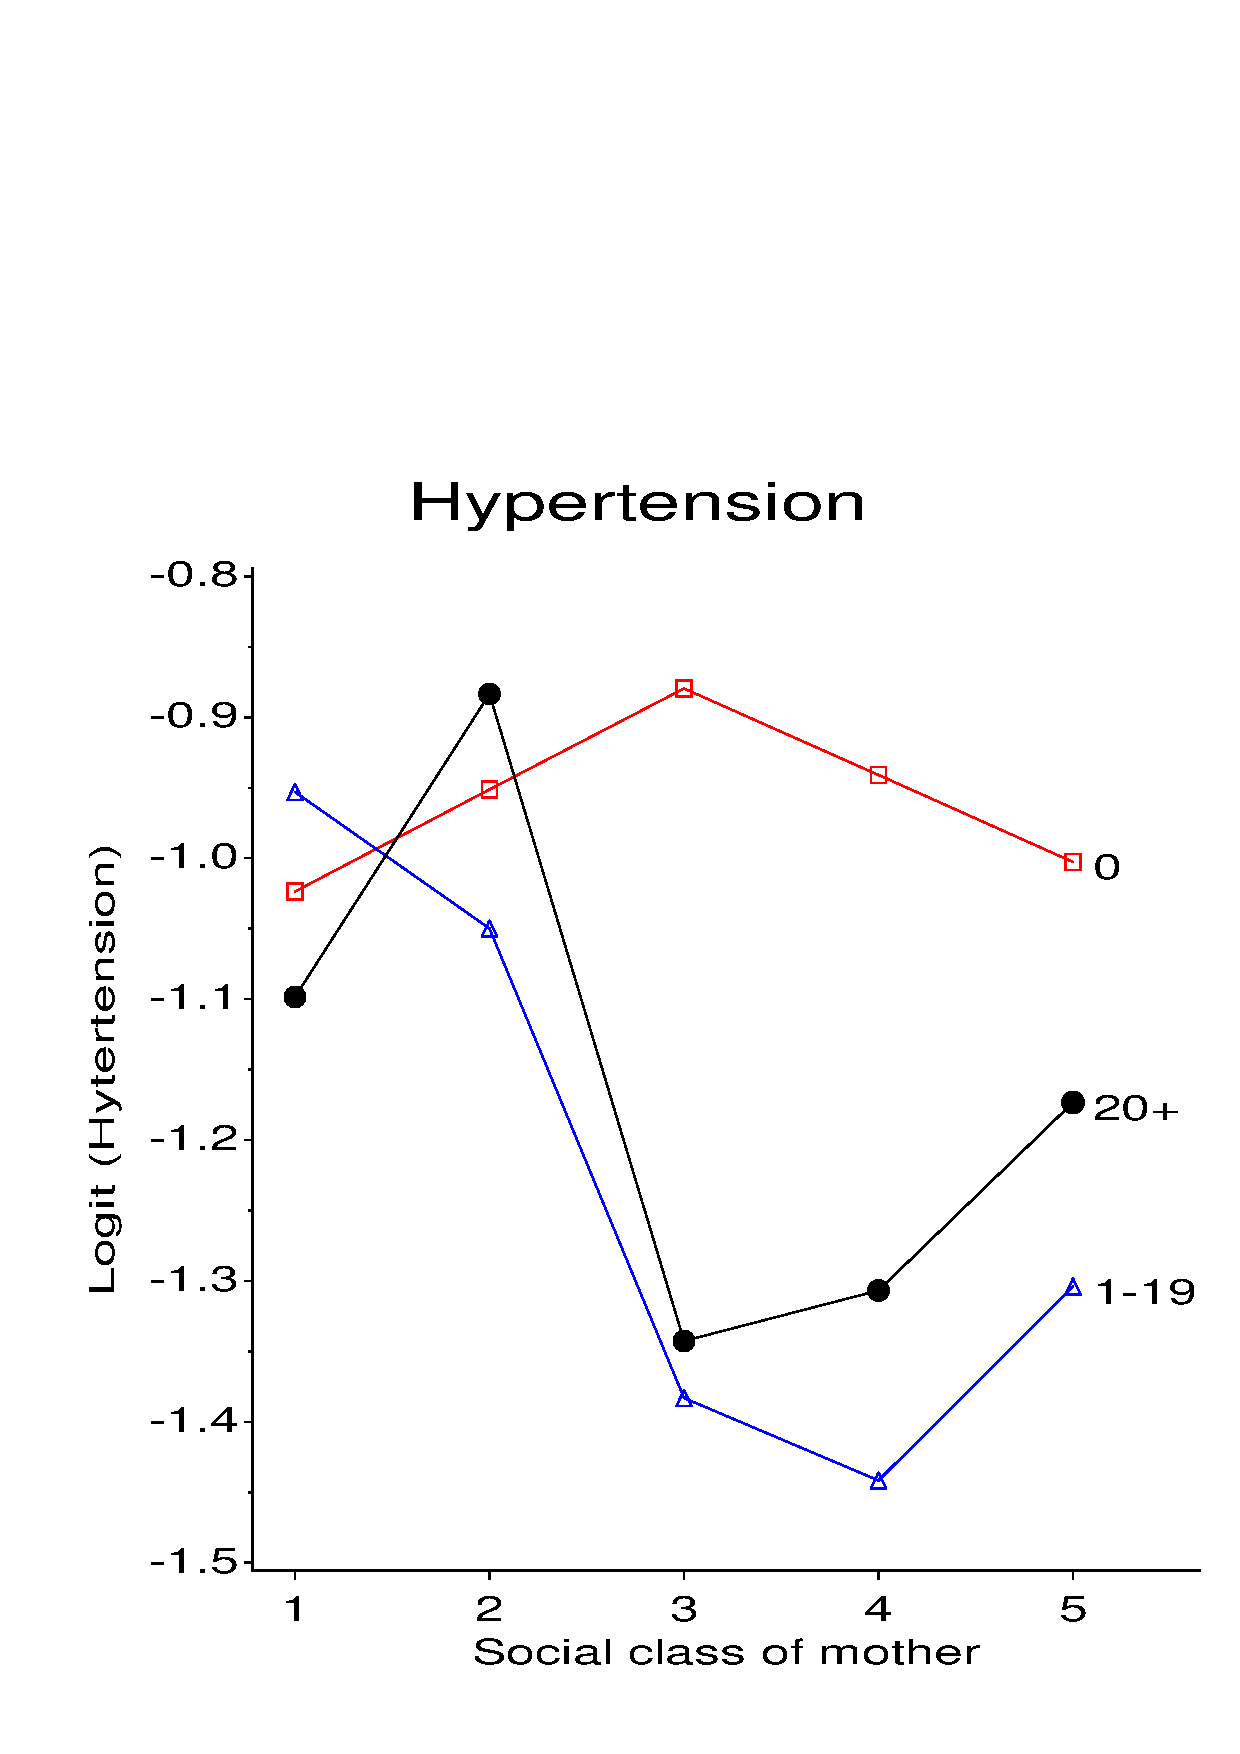
\includegraphics[width=1\linewidth]{tox11}
 \end{minipage}%
 \hfill
 \begin{minipage}[t]{.49\linewidth}
  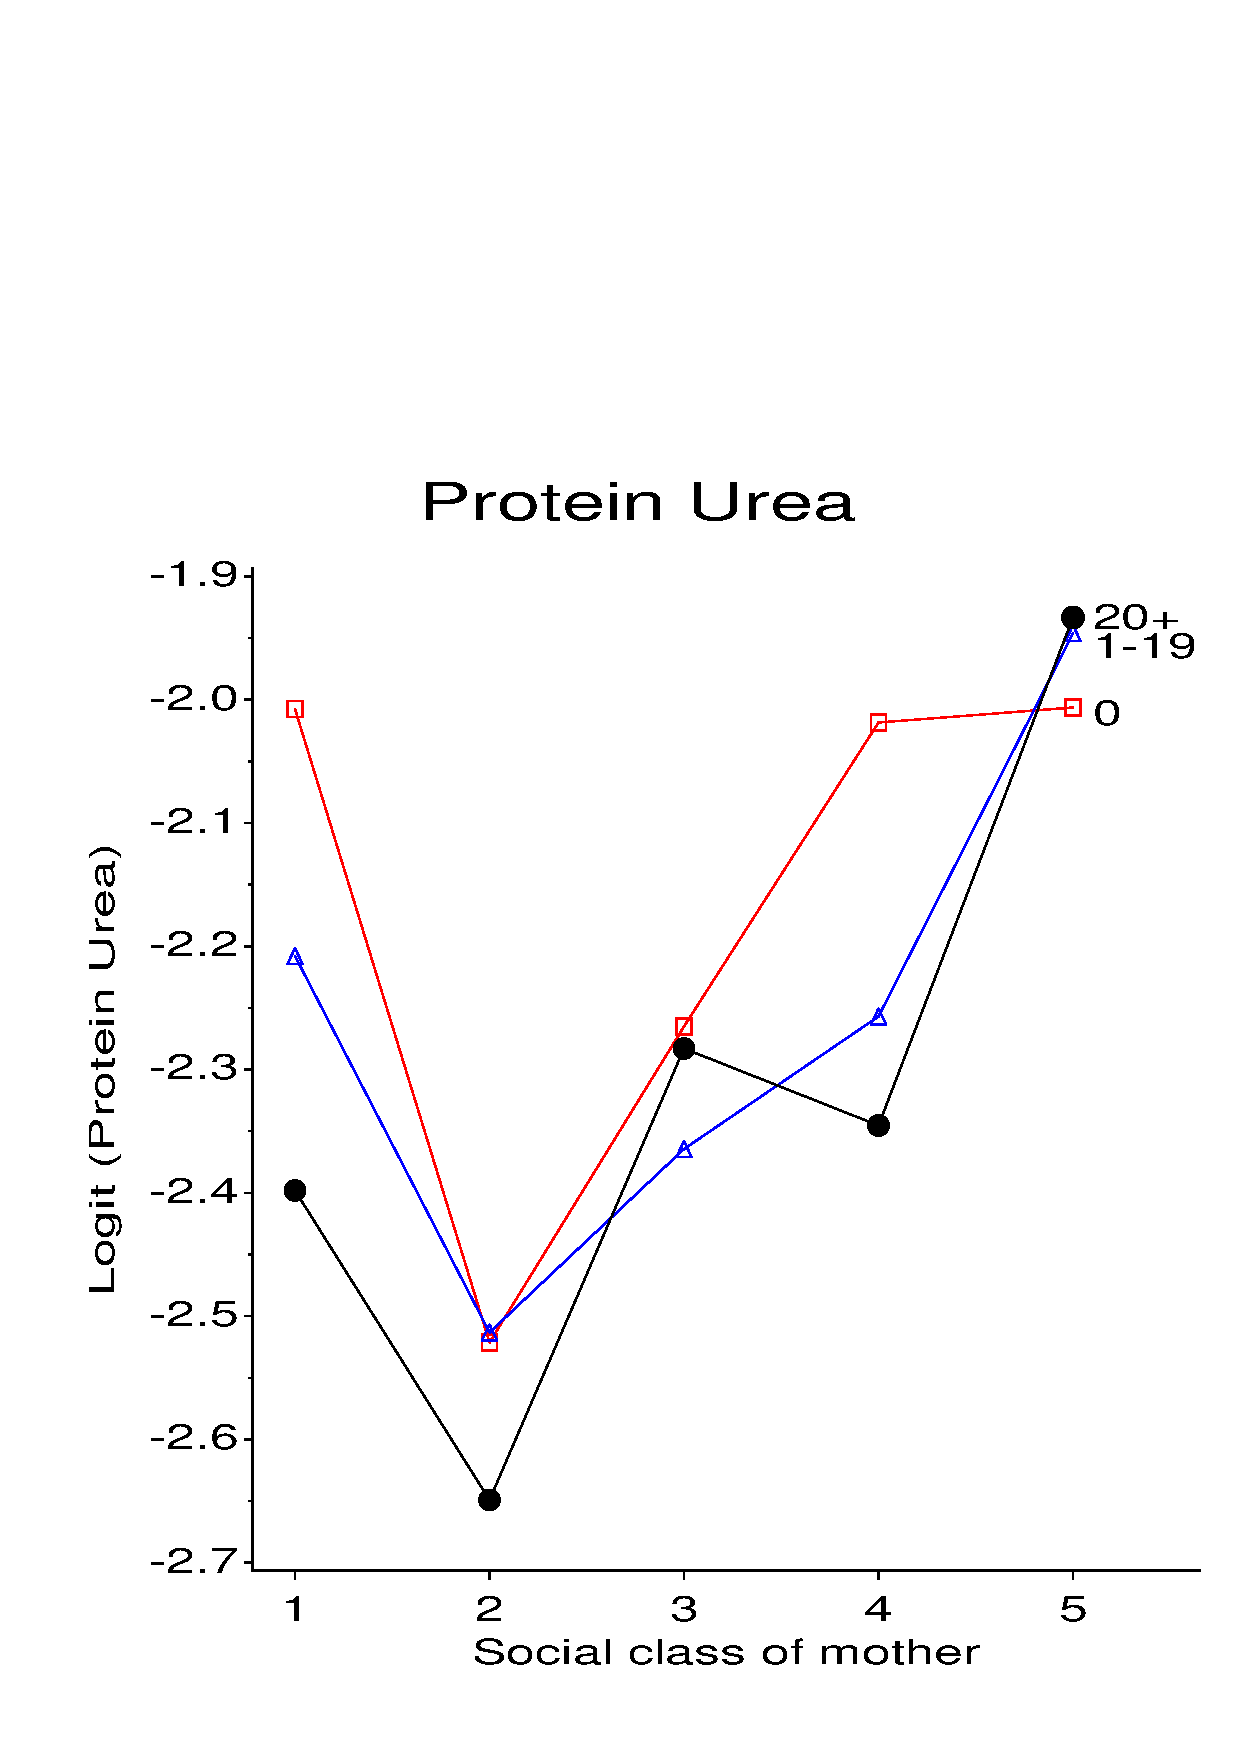
\includegraphics[width=1\linewidth]{tox12}
 \end{minipage}
 \caption{Logits for hypertension and for protein urea, by social class and smoking}\label{fig:tox11}
\end{figure}

From \figref{fig:tox11} it may be seen that the prevalence of these
symptoms has a possibly complex relation to social class and smoking.
However, the mosaic for these predictors in \figref{fig:tox41} has shown
us that several of the class-smoking categories are quite small
(particularly heavy smokers in Class 1)
so the response effects for these classes will be poorly estimated.
Taking this into account,
we suspect that protein urea varies with social class, but not with
smoking, while the prevalence of hypertension may truly vary with neither,
just one, or both of these predictors.

The association between the response symptoms,
shown in \figref{fig:tox13}
is clearer, once we take the variation in sample sizes into account.
Except for the heavy smokers, particularly  in social classes 1 and 2, the log odds ratio
appears to be relatively constant.
%% one figure
\begin{figure}[htb]
  \centering
  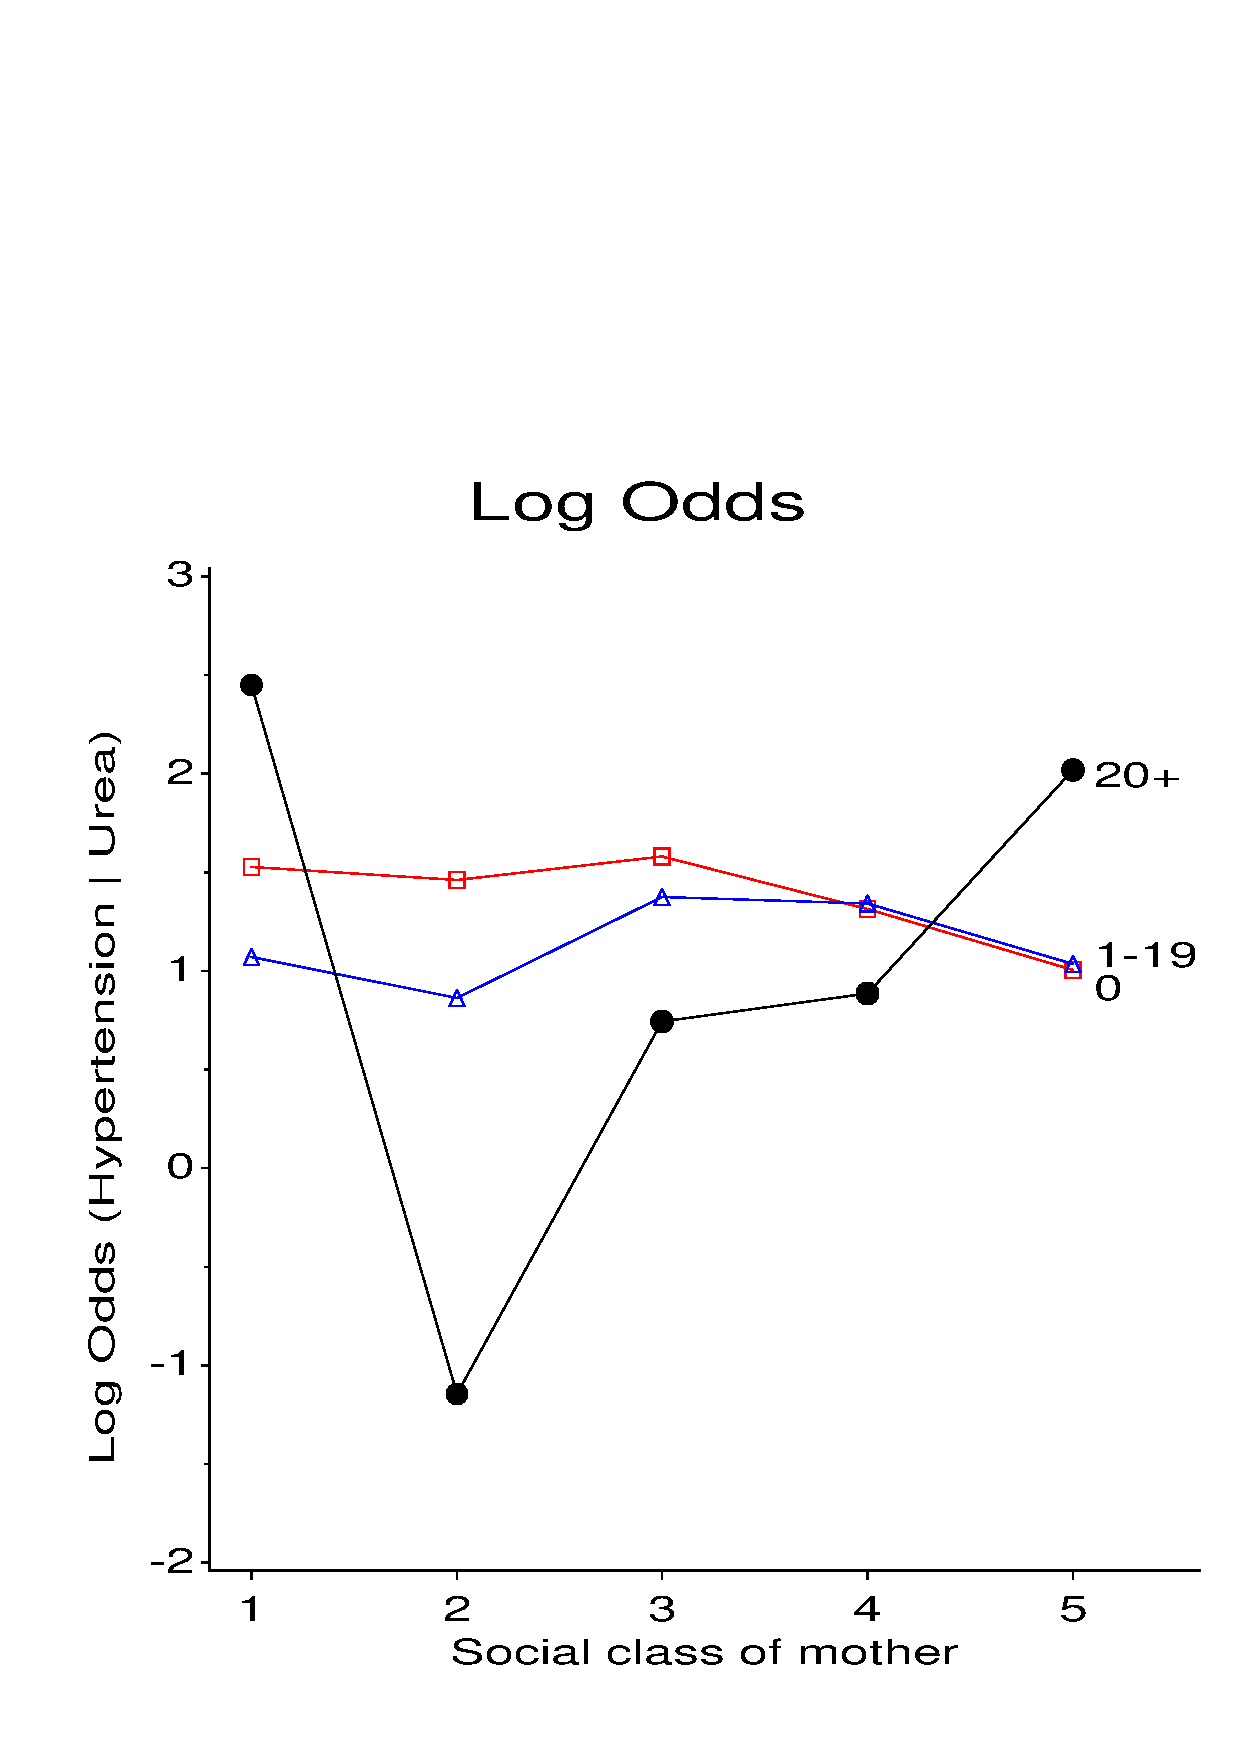
\includegraphics[scale=.4]{tox13}
  \caption{Log odds ratio for hypertension, given protein urea, by social class and smoking}%
  \label{fig:tox13}
\end{figure}

When there are no quantitative predictors, and when the odds ratio is
relatively constant, it is easier to fit ordinary \loglin\ models
than to use the bivariate logit formulation of the previous example.

We fit these models using the \stmt{LOGLIN}{CATMOD} as shown below.
There are two zero cells in \tabref{tab:toxtab}.
In the \loglin\ formulation \PROC{CATMOD} treats these as structural
zeros, so we first replace the zeros with a small positive number.
The minimal model, $[CS] [H] [U]$ fits the marginal association of the
numbers in each Class-Smoking category, but asserts that the responses,
$H$ and $U$ are independent, which we have already seen is contradicted
by the data.  We take $[CS] [HU]$ as the null model (Model 0), asserting no relation
between response and predictor variables.
%% input: /users/faculty/friendly/sasuser/catdata/tox2l.sas
%% last modified: 19-Nov-98  9:23
\begin{listing}
%include catdata(toxaemia);
data toxaemia;
   set toxaemia;
   if count=0 then count=1E-10;

*-- Loglinear models;
proc catmod order=data
            data=toxaemia;
   weight count;
   model hyper*urea*class*smoke =  _response_ /
      ml noiter noresponse noprofile nodesign;
   loglin  class|smoke hyper urea / title='Model -1: CS  H  U';
run;
   loglin  class|smoke hyper|urea / title='Model 0: CS  HU';
run;
   loglin  class|smoke  hyper|urea  hyper|smoke  urea|class /
       title='Model 1: CS  HU  SH  CU';
run;
   loglin  class|smoke|hyper|urea @2 /
       title='Model 2: CS  CH  CU  HU  SH  CU';
run;
   loglin class|smoke|hyper  class|urea  hyper|urea /
       title='Model 3: CSH  CU  HU';
run;
   loglin class|smoke|hyper  class|urea  smoke|urea  hyper|urea /
       title='Model 4: CSH  CU  SU  HU';
run;
   loglin class|smoke|hyper  class|smoke|urea  hyper|urea /
       title='Model 5: CSH  CSU  HU';
run;
\end{listing}


The fit statistics and some model selection criteria for these and other
models are shown in \tabref{tab:toxmod}.
The large residual $G^2$ for Model 0 (179.03 on 42 df) indicates substantial
associations between the responses and explanatory variables.
Model 1 adds the simple dependence of hypertension on smoking ($[SH]$) and that of urea on class ($[CU]$); Model 2 includes all two-way terms.
In Model 3, hypertension is allowed to depend on both class and smoking
jointly ($[CSH]$). In Model 4 an additional dependence of
urea on smoking ($[SU]$) is included, while in Model 5 urea depends on
class and smoking jointly ($[CSU]$).
\begin{table}[htb]
 \caption{Loglinear models fit to toxaemia data}\label{tab:toxmod}
 \begin{center}
 \begin{tabular}{rl rrrrrrr}
  \hline
  Model & Terms         & df & \chisq & $p$-value & \chisq /df & AIC & $R^2$ & Adj. $R^2$ \\ 
  \hline
 -1 & CS H U            & 43 & 672.85 & 0.0000 & 15.65 & 586.85 & . & . \\ 
  0 & CS HU             & 42 & 179.03 & 0.0000 & 4.26 & 95.03 & 0.000 & 0.000 \\ 
  1 & CS HU SH CU       & 36 & 46.12 & 0.1203 & 1.28 & -25.88 & 0.742 & 0.699 \\ 
  2 & CS CH CU HU SH CU & 30 & 40.47 & 0.0960 & 1.35 & -19.53 & 0.774 & 0.684 \\ 
  3 & CSH CU HU         & 24 & 26.00 & 0.3529 & 1.08 & -22.00 & 0.855 & 0.746 \\ 
  4 & CSH CU SU HU      & 22 & 25.84 & 0.2588 & 1.17 & -18.16 & 0.856 & 0.724 \\ 
  5 & CSH CSU HU        & 14 & 22.29 & 0.0729 & 1.59 & -5.71 & 0.875 & 0.626 \\ 
  6 & CSH CSU SHU       & 12 & 15.65 & 0.2079 & 1.30 & -8.35 & 0.913 & 0.694 \\ 
  7 & CSH CSU CHU SHU   & 8 & 12.68 & 0.1233 & 1.59 & -3.32 & 0.929 & 0.628 \\ 
  8 & CSHU              & 0 & 0.00 & . & . & 0.00 & 1.000 & . \\ 
  \hline
 \end{tabular}
 \end{center}
\end{table}


None of these models contain three-way terms involving both $H$ and $U$,
so these models assume that the log odds ratio for hypertension given urea
is constant over the explanatory variables.
Recalling the partial mosaics (\figref{fig:tox42} and \figref{fig:tox43})  Models 6 and 7 add terms
which allow the odds ratio to vary, first with smoking ($[SHU]$), then
with class ($[CHU]$) as well.

How do we choose among these models?  Model 1 is the smallest whose deviance
is non-significant. Models 3 and 4 both have a smaller ratio of \chisq\/df.
For comparing nested models, we can also examine the change in deviance as
terms are added (or dropped).  Thus, going from Model 1 to Model 2
decreases the deviance by 5.65 on 6 df, while the step from Model 2 to Model 3
gives a decrease of 14.47, also on 6 df.  The AIC statistic, balancing
parsimony and goodness-of-fit, has its minimum value for Model 1,
which we adopt here for this example.

Whatever model is chosen, as a final step, it is important to determine what
that model implies about the original research questions.
Because our focus here is on the prevalence of each symptom, and their
association, it is helpful to graph the fitted logits and log odds ratios
implied by the model, as we did in \figref{fig:ash21} and \figref{fig:ash22}.

In \exref{ex:ashford} we fit the bivariate logit model, for which the
response functions were the desired logits and log odds.
Here, where we have fit ordinary \loglin\ models, the fitted logits
can be calculated from the fitted frequencies.
To obtain predicted frequencies under Model 1, we use the option
\pname{PRED=FREQ} on the \stmt{MODEL}{CATMOD}.
%% input: /users/faculty/friendly/sasuser/catdata/tox2.sas
%% last modified: 19-Nov-98 15:21
\begin{listing}
proc catmod order=data data=toxaemia;
   weight count;
   response  / out=predict;
   model hyper*urea*class*smoke =  _response_ / pred=freq
      ml noiter noresponse noprofile nodesign;
   loglin  class|smoke hyper|urea hyper|smoke urea|class /
       title='Model 1: CS  HU  SH  CU';
\end{listing}

Then, the observed and fitted frequencies can be extracted from
the \ODS, and rearranged so that logits and log odds
may be calculated.
%% input: /users/faculty/friendly/sasuser/catdata/tox2.sas
%% last modified: 19-Nov-98 15:27
\begin{listing}
data predict;
   set predict;
   where (_type_='FREQ');
   drop _sample_ _number_ _type_;
proc sort data=predict;
   by class smoke hyper urea;

proc transpose data=predict out=fit(drop=_label_) prefix=fit;
   by class smoke;
   var _pred_;
proc transpose data=predict out=obs(drop=_label_) prefix=obs;
   by class smoke;
   var _obs_;

data pred;
   merge fit obs;
   drop _name_;
   array f\{4\} fit1-fit4;   *-- Fitted frequencies;
   array o\{4\} obs1-obs4;   *-- Observed frequencies;
   
   fhyper = log( (f[1] + f[2] + .5) / (f[3] + f[4] + .5) );
   furea =  log( (f[1] + f[3] + .5) / (f[2] + f[4] + .5) );
   fodds=  log( ((f[1]+.5)*(f[4]+.5))/((f[2]+.5)*(f[3]+.5)) );
   
   ohyper = log( (o[1] + o[2] + .5) / (o[3] + o[4] + .5) );
   ourea =  log( (o[1] + o[3] + .5) / (o[2] + o[4] + .5) );
   oodds=  log( ((o[1]+.5)*(o[4]+.5))/((o[2]+.5)*(o[3]+.5)) );
   
   label fhyper = 'Logit (Hytertension)'
      furea =   'Logit (Protein Urea)'
      fodds = 'Log Odds (Hypertension | Urea)';
   format smoke smoke.;
\end{listing}

%% one figure
\begin{figure}[htb]
  \centering
  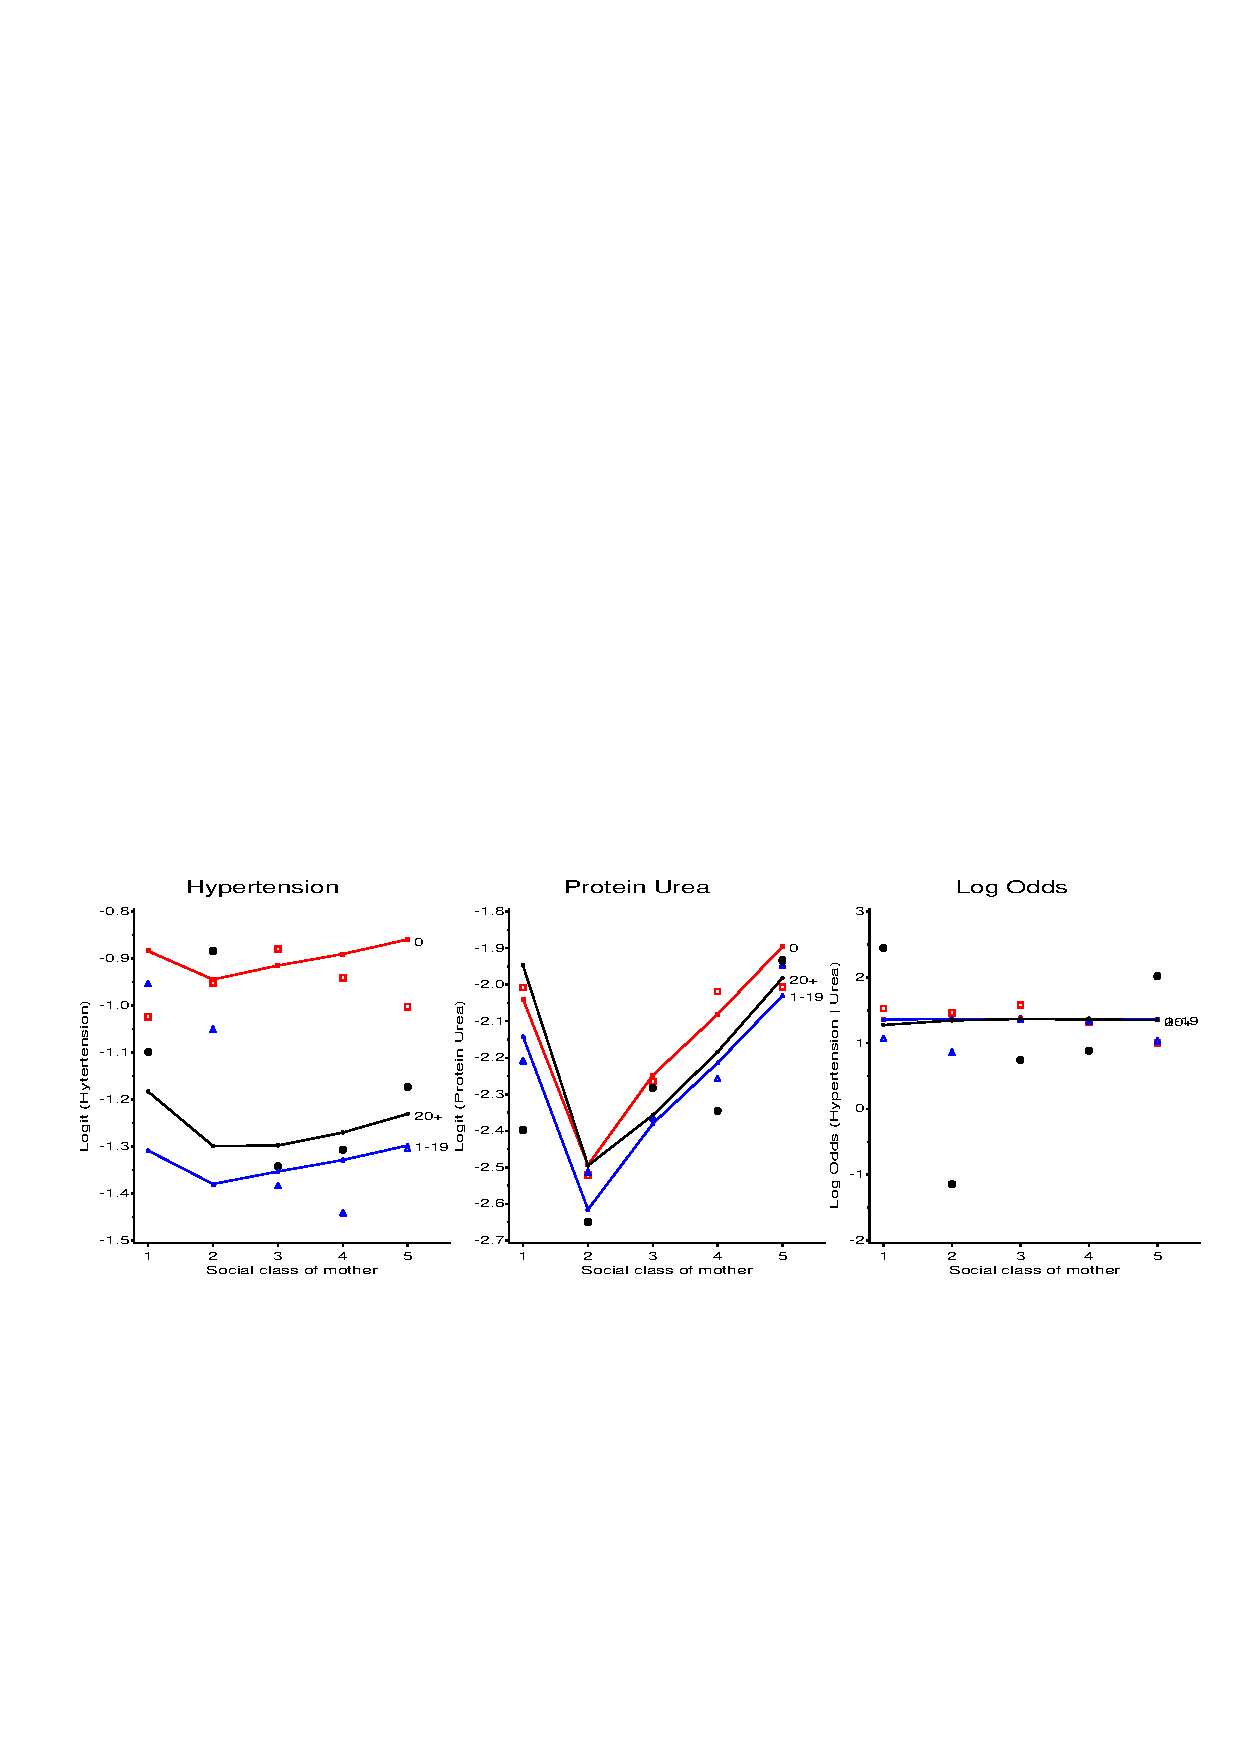
\includegraphics[width=\textwidth,clip]{tox2}
  \caption{Toxaemia data: Observed and fitted logits and log odds ratios for Model 1: $[CS] [HU] [SH] [CU]$}%
  \label{fig:tox2}
\end{figure}
Finally, each measure is plotted separately, showing the fitted values
with curves and the observed values with points.  The statements
below are repeated for urea and for log odds.  The three graphs are
shown in \figref{fig:tox2}.
%% input: /users/faculty/friendly/sasuser/catdata/tox2.sas
%% last modified: 19-Nov-98 15:29
\begin{listing}
%label(data=pred, x=class, y=fhyper, subset=(class=5),
   text=put(smoke, smoke.), pos=6, xoff=.1, out=lab);

%points(data=pred, x=class, y=ohyper, 
   symbol=scan('square triangle dot',smoke),
   color=scan('red blue black', smoke), size=2, out=_pts_);
data lab;
   set lab _pts_;

proc gplot data=pred;
   plot fhyper  * class = smoke / anno=lab nolegend
      vaxis=axis1 haxis=asix2 hm=0 vm=1;
   symbol1 v=square   h=1 i=join c=red;
   symbol2 v=triangle h=1 i=join c=blue;
   symbol3 v=dot      h=1 i=join c=black;
   axis1 label=(a=90) order=(-1.5 to -0.8 by .1);
   axis2 offset=(3,9);
   title 'Hypertension';
\end{listing}

We can see from \figref{fig:tox2} that the fitted log odds ratio is in fact
nearly constant,
while the log odds for hypertension depends mainly on smoking, while
that for protein urea depends mainly on social class.
Yet, the great variability of the observed points around the fitted
curves indicates that these relationships are not well-determined.
Adding error bars showing the standard error around each fitted point
would indicate that the data conforms as closely to the model as
can be expected, given the widely different sample sizes.
However, this would make the plots more complex, and so was omitted
here.
In addition to showing the pattern of the results according to the fitted
model, such graphs also help us to appreciate the model's limitations.
\end{Example}

